\documentclass[11pt]{beamer}
\usepackage{talk}

\begin{document}

\title{A quick intro to MEGA's open-source SDK}
\author{Christian Blume}
\date{December 3, 2019} 

\begin{frame}
\titlepage
\end{frame}

\begin{frame}[fragile]
\frametitle{What is MEGA?}
\bigskip
\bigskip

\begin{itemize}
\item MEGA is a cloud storage provider using end-to-end encryption
\item The encryption key is in the user's hand (their password)
\item MEGA is all about the user's privacy
\end{itemize}
\bigskip

\begin{center}
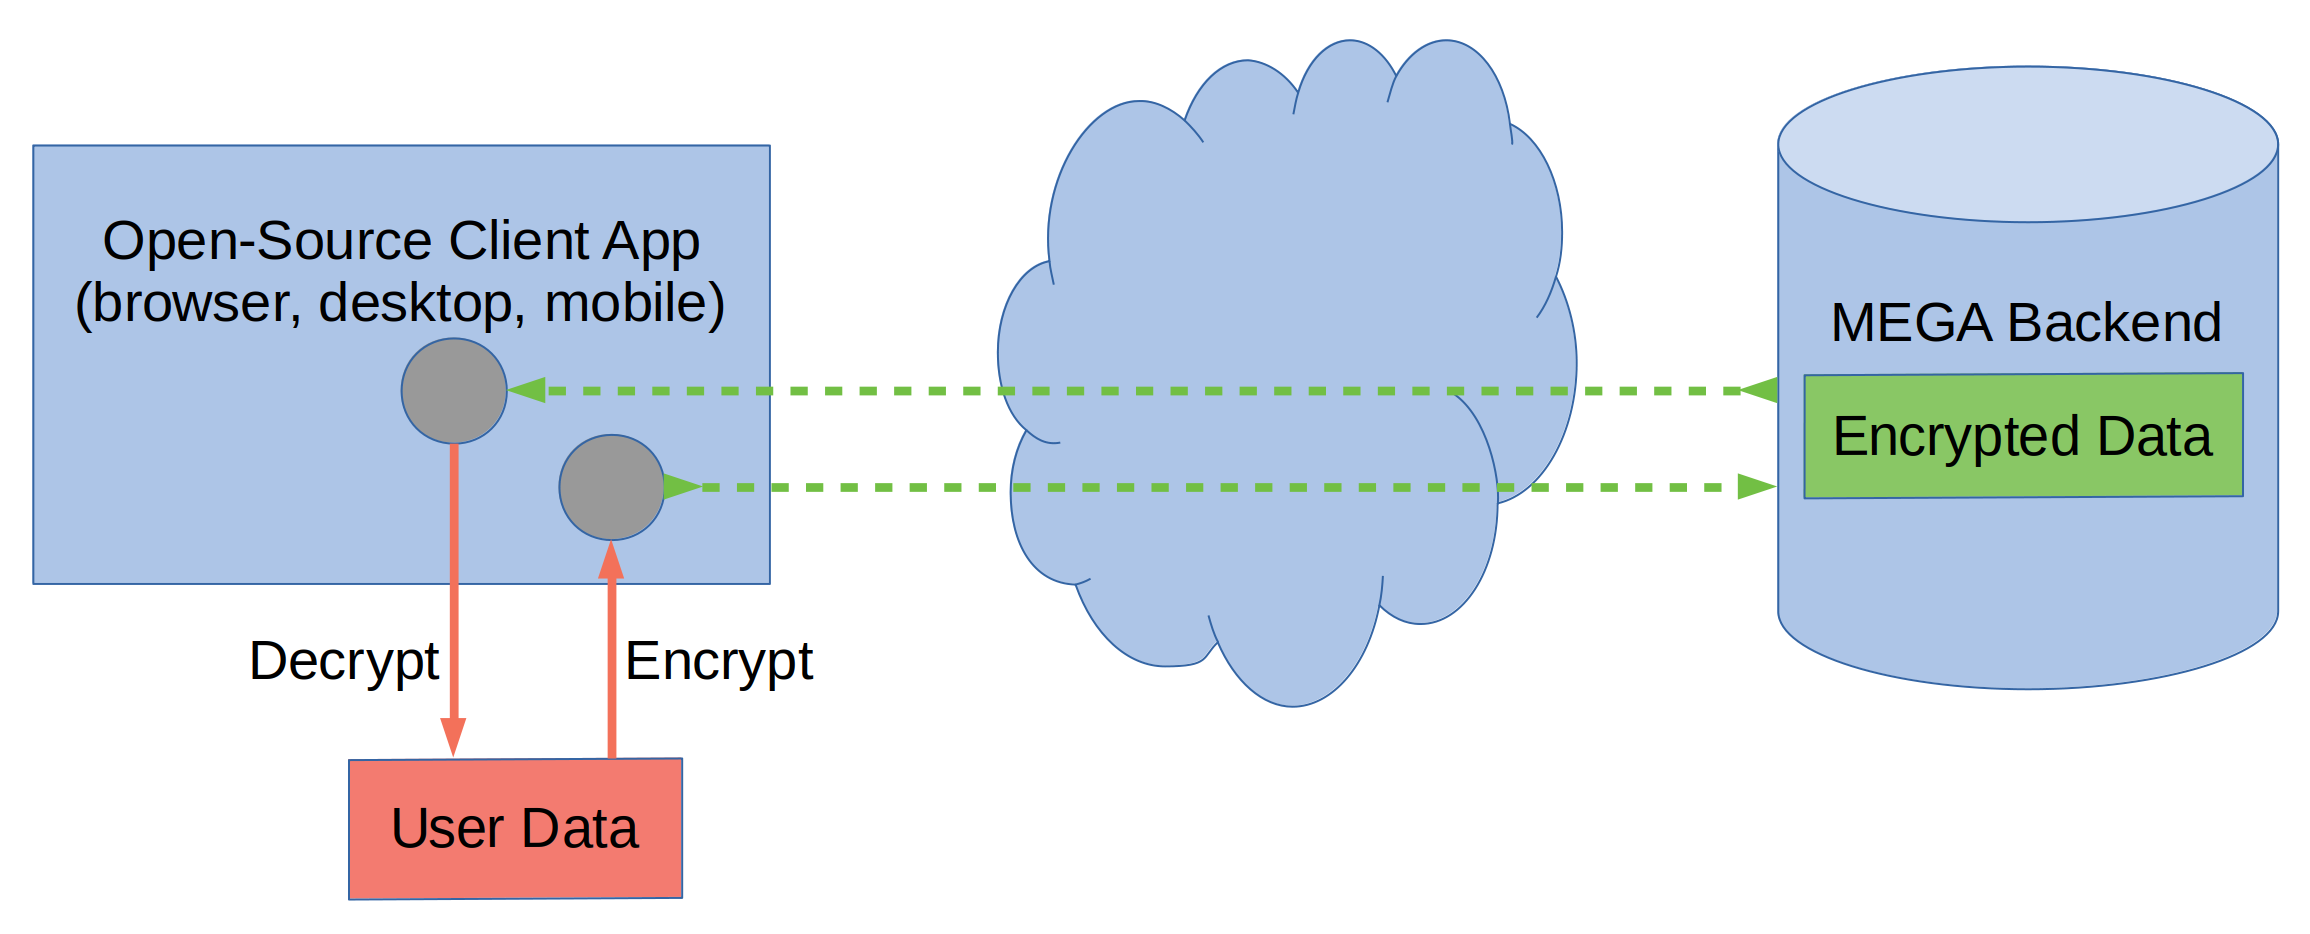
\includegraphics[width=1\textwidth]{img/general}
\end{center}

\end{frame}

\begin{frame}[fragile]
\frametitle{What is MEGA's SDK?}
\bigskip

\begin{itemize}
\setlength\itemsep{1em}
\item A C\texttt{++} layer to fully control your MEGA account
\item Common functionality shared across all native apps
\item Provides bindings to Objective-C, Java, Perl, Python, etc
\item Abstracts: Encyrption, account management, networking, fileystem
  access, synchronization, etc
\item Two parts: \textit{Core} and \textit{Intermediate Layer} (MegaApi)
\end{itemize}
\end{frame}

\begin{frame}[fragile]
\frametitle{What is MEGA's SDK? (cont)}
\bigskip

\begin{center}
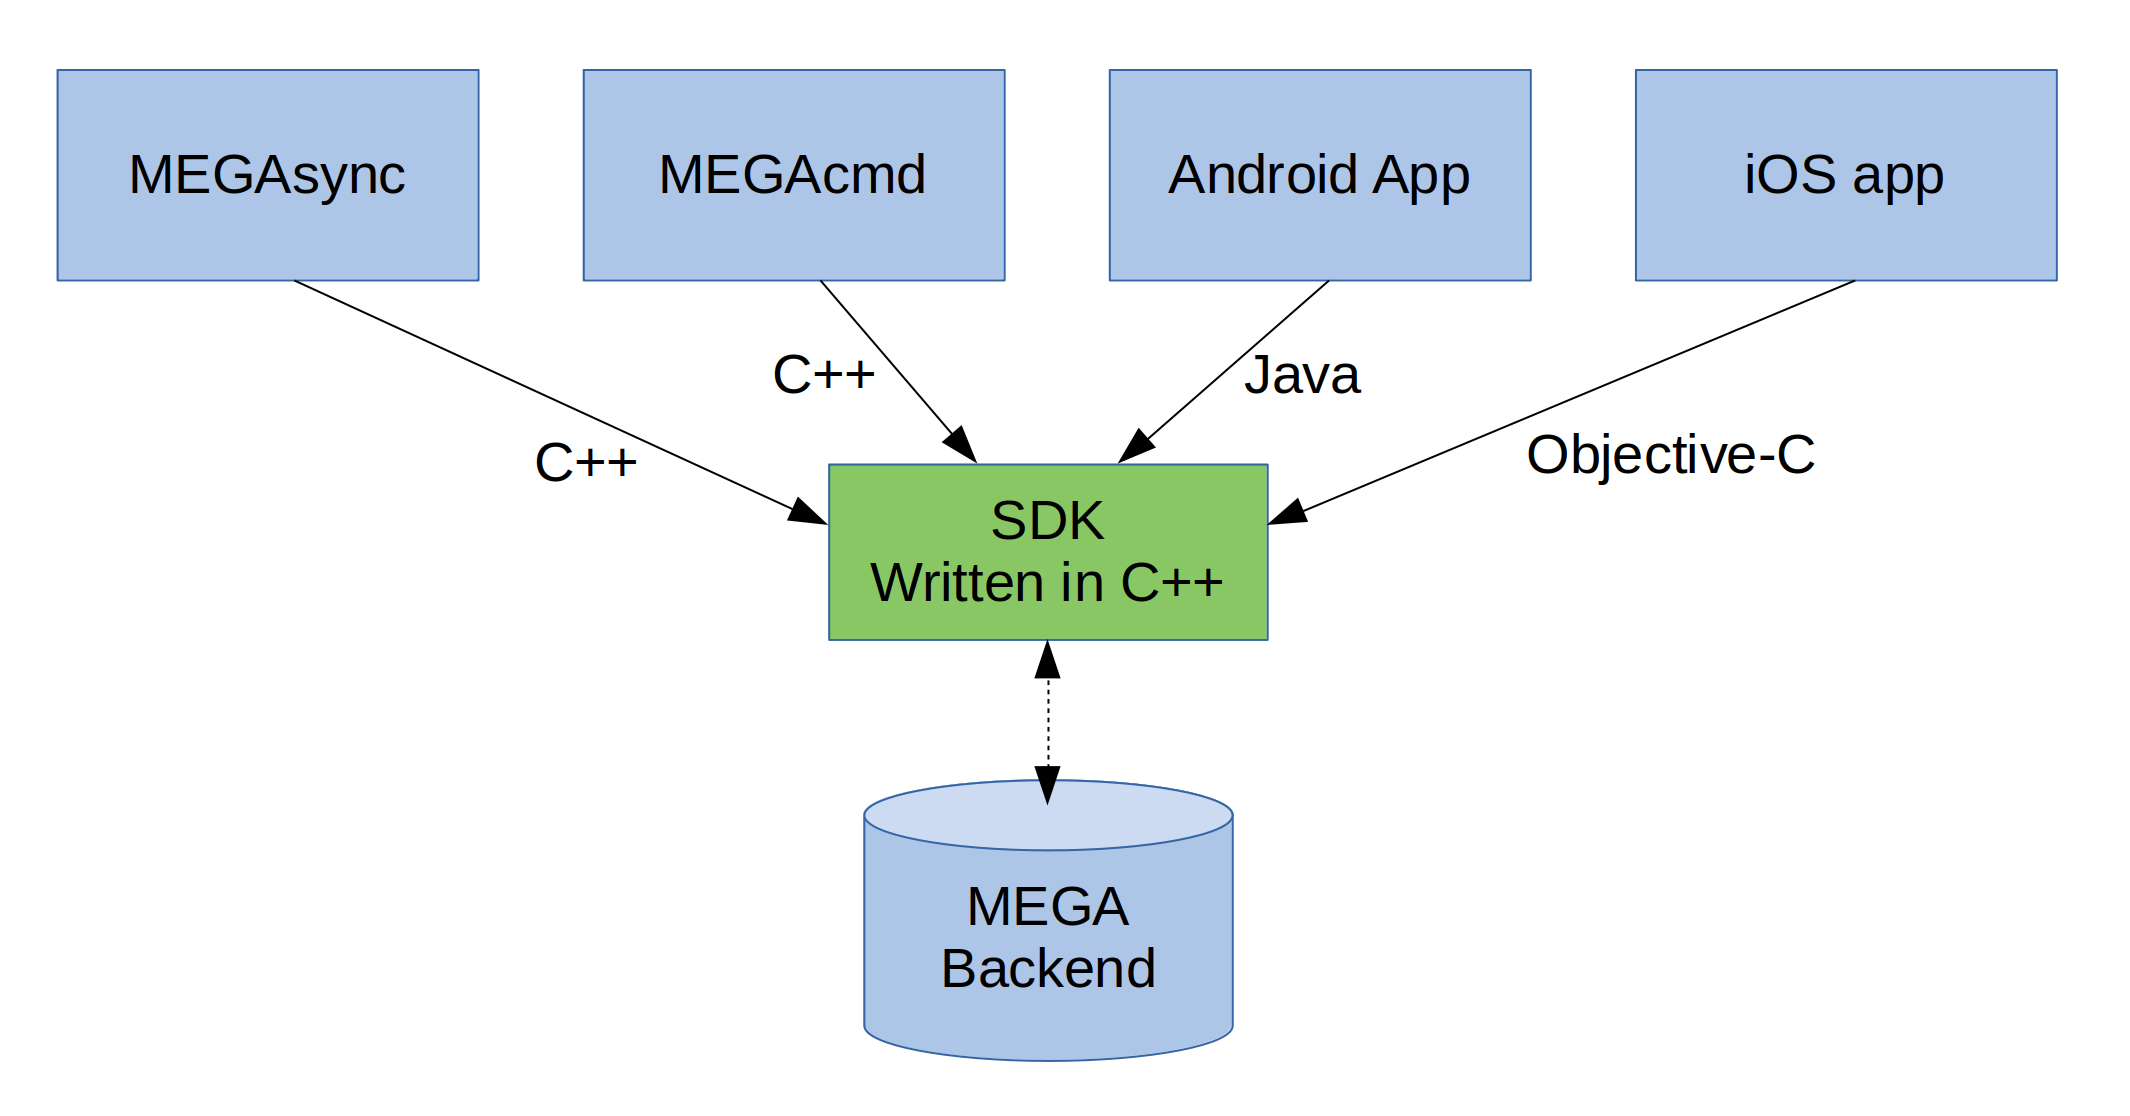
\includegraphics[width=1\textwidth]{img/sdk}
\end{center}
\medskip

\url{https://github.com/meganz/sdk}
\end{frame}

\begin{frame}[fragile]
\frametitle{The SDK's API}

\begin{lstlisting}
class MegaApi;  // main entry point
\end{lstlisting}
\bigskip

\begin{itemize}
\item Every instance spins up a worker thread processing events
\item MegaApi functions are either synchronous or asynchronous
\item An async function enqueues the request and processes it on the SDK thread
\item Async results are communicated through a listener interface
\end{itemize}
\bigskip

\begin{lstlisting}
// For example:
void MegaApi::login(const char* email, const char* password, MegaRequestListener *listener = NULL);
\end{lstlisting}

\end{frame}

\begin{frame}[fragile]
\frametitle{Demo time}

Problem: List all files and directories in your MEGA account.
\bigskip
\bigskip

Simple command-line tool:

\url{https://github.com/bloomen/list-mega-account}
\bigskip
\bigskip

In a nutshell:
\begin{itemize}
\item Log into account
\item Fetch all remote nodes
\item Print all files and directories
\item Log out
\end{itemize}

\end{frame}

\end{document}
